\documentclass{article}
\usepackage{fullpage,amsmath,amsthm,graphicx,enumitem,amssymb}
\usepackage[hidelinks]{hyperref}
\theoremstyle{definition}
\newtheorem{thm}{Theorem}
\newtheorem{question}[thm]{Question}
\newenvironment{solution}{\noindent\textit{Solution:}}{}
\usepackage{etoolbox}

\newcommand{\reals}{\mathbb{R}}

\title{ASEN 5519-003 Decision Making under Uncertainty\\
       Homework 3: Online MDP Methods}

\begin{document}

\maketitle

\section{Conceptual Questions}

\begin{question} (20 pts) Do similar $Q$ values imply similar rewards?

    In the proof for Lemma 5 of the Sparse Sampling paper by Kearns, Mansour, and Ng,\footnote{\url{https://www.cis.upenn.edu/~mkearns/papers/sparsesampling-journal.pdf}; Note: you do not need to read the paper to complete the problem.}, the authors make the following claim:
    \begin{quote}
    If a policy $\pi$ satisfies $|Q^*(s, \pi^*(s)) - Q^*(s, \pi(s))| \leq \beta$ for all $s \in \mathcal{S}$, then it immediately follows that $|\mathcal{R}(s, \pi^*(s)) - \mathcal{R}(s, \pi(s))| \leq \beta$.
    \end{quote}
    In this exercise, you will demonstrate that this claim is mistaken. Consider the MDP below:
    \begin{center}
        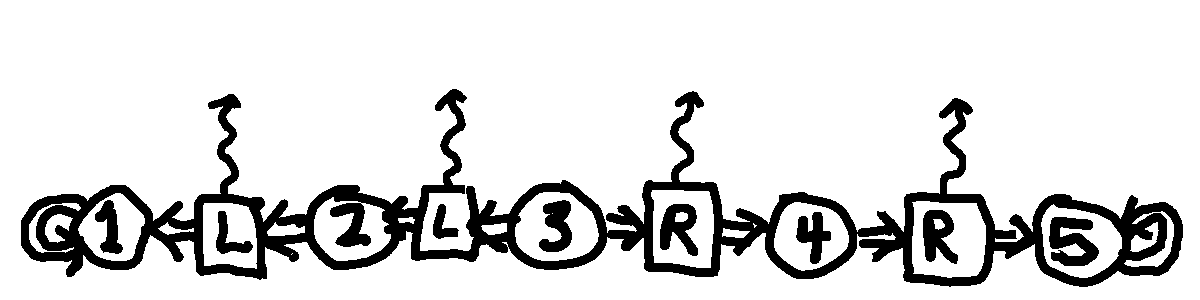
\includegraphics[width=0.7\textwidth]{hand_mdp.pdf}
    \end{center}
    The state space is $S = \{1, \ldots, 5\}$ and the action space is $A = \{L, R\}$ (but not all actions are available from each state). Transitions are deterministic as shown. The discount factor is $\gamma=0.9$.

    Choose a reward function, $\mathcal{R}$, (i.e. values for the squiggly arrows), a policy, $\pi$, and a value $\beta$ that constitute a counterexample to the claim above. Justify your answer.
\end{question}

\section{Exercises}
    \texttt{HW3.DenseGridWorld()} generates a 60x60 grid world MDP. There is a reward of +100 every 20 cells, i.e. at [20,20], [20,40], [40,20], etc. Once the agent reaches one of these reward cells, or an edge cell, the problem terminates. All cells also have a cost. Only a generative transition model is available. You will use the following functions from POMDPs.jl to interact with this problem (or larger versions) in the rest of this assignment:
    \begin{itemize}[nosep]
        \item \texttt{actions(m)}
        \item \texttt{@gen(:sp, :r)(m, s, a)}
        \item \texttt{isterminal(m, s)}
        \item \texttt{discount(m)}
        \item \texttt{statetype(m)}
        \item \texttt{actiontype(m)}
    \end{itemize}

\begin{samepage}
\begin{question} (15 pts) Monte Carlo Policy Evaluation
    \begin{enumerate}[label=\alph*)]
        \item Write a rollout simulation function for an MDP starting with the following code:
            \begin{verbatim}
        r_total = 0.0
        t = 0
        while !isterminal(mdp, s) && t < max_steps
            a = :down # replace this with a policy
            s, r = @gen(:sp,:r)(mdp, s, a)
            r_total += discount(m)^t*r
            t += 1
        end
                \end{verbatim} Use this function to perform a Monte Carlo evaluation of a uniform random policy on an MDP created with \texttt{HW3.DenseGridWorld(seed=3)}. Report the mean discounted reward estimate and standard error of the mean (SEM). Run enough simulations so that the SEM is less than 5.
         \item Create a heuristic policy that improves upon the random policy by at least 50 reward units. Report the mean and standard error from a Monte Carlo evaluation.
    \end{enumerate}
\end{question}
\end{samepage}

\begin{question} \label{q:mcts} (20 pts) Monte Carlo Tree Search
    
    Write code that performs 7 iterations of Monte Carlo Tree Search on an MDP created with \\
    \texttt{HW3.DenseGridWorld(seed=4)},
    starting at state $(19, 19)$. You will need to produce three dictionaries:
    \begin{itemize}[noitemsep]
        \item \texttt{Q} maps $(s, a)$ tuples to Q value estimates.
        \item \texttt{N} maps $(s, a)$ tuples to N, the number of times the node has been tried.
        \item \texttt{t} maps $(s, a, s')$ tuples to the number of times that transition was generated during construction of the tree.
    \end{itemize}
    Then visualize the resulting tree with \texttt{HW3.visualize\_tree(Q, N, t, SA[19, 19])}\footnote{\texttt{SA} is from the \texttt{StaticArrays.jl} package.}. \textbf{Submit an image of the tree, the code used to generate it, and a few sentences describing the tree after 7 iterations} (e.g. which actions have the highest Q values? Does this make sense?).
    
\end{question}

\begin{question}
    (15 pts) Planning with MCTS

    Use your Monte Carlo tree search from Question~\ref{q:mcts} to plan online in the simulation loop. Limit the planning time to 50ms. Evaluate the MCTS planner with 100 100-step Monte Carlo simulations. Report the mean accumulated reward and standard error of the mean, along with a typical number of iterations that MCTS was able to complete each time it chose an action\footnote{You can determine a typical number of iterations by just printing out the number; you don't need to keep careful statistics unless you want to}.
\end{question}

\section{Challenge Problem}

\begin{question}
    (10 pts code and description, 20 pts score) Fast Online Planning
    
    Create a function \texttt{select\_action(m,s)} that takes in a $100 \times 100$ \texttt{DenseGridWorld}, \texttt{m}, and a state \texttt{s}, and returns a near-optimal action within 50ms. You may wish to base this code on the MCTS code that you wrote for Question~\ref{q:mcts}. Evaluate this function with \texttt{HW3.evaluate} and \textbf{submit the resulting \texttt{json} file along with the code and a one paragraph to one page description of your approach}, including tuning parameters that worked well, the rollout policy, etc. A score of 50 will receive full credit. There are no restrictions on this problem - you may wish to use a different algorithm, multithreading, etc. Starter code on github will give suggestions for timing and other details.
\end{question}

\end{document}
